\documentclass[11pt,a4paper]{article}

\usepackage[utf8]{inputenc}
\usepackage[margin=0.85in]{geometry}
\usepackage{amsmath,amssymb,amsfonts}
\usepackage{graphicx}
\usepackage{booktabs}
\usepackage{xcolor}
\usepackage{subcaption}
\usepackage{float}
\usepackage{hyperref}
\usepackage{listings}
\usepackage{microtype}
\usepackage{algorithm}
\usepackage{algpseudocode}

\hypersetup{
    colorlinks=true,
    linkcolor=blue!70!black,
    citecolor=blue!70!black,
    urlcolor=blue!70!black
}

\definecolor{codegreen}{rgb}{0,0.6,0}
\definecolor{codegray}{rgb}{0.5,0.5,0.5}
\definecolor{codepurple}{rgb}{0.58,0,0.82}
\definecolor{backcolour}{rgb}{0.96,0.96,0.96}

\lstdefinestyle{mystyle}{
    backgroundcolor=\color{backcolour},   
    commentstyle=\color{codegreen},
    keywordstyle=\color{magenta},
    numberstyle=\tiny\color{codegray},
    stringstyle=\color{codepurple},
    basicstyle=\ttfamily\footnotesize,
    breakatwhitespace=false,         
    breaklines=true,                 
    captionpos=b,                    
    keepspaces=true,                 
    numbers=left,                    
    numbersep=5pt,                  
    showspaces=false,                
    showstringspaces=false,
    showtabs=false,                  
    tabsize=2
}
\lstset{style=mystyle}

\lstdefinestyle{console}{
    backgroundcolor=\color{backcolour},
    basicstyle=\ttfamily\small,
    breaklines=true,
    columns=fullflexible,
    keepspaces=true,
    numbers=none,
    frame=single,
    rulecolor=\color{black!20}
}

\begin{document}

\graphicspath{{images/}}

\begin{titlepage}
\centering

\includegraphics[width=0.68\textwidth]{logo.png}\\[1cm]

{\Huge \textbf{Assignment 2}}\\[0.5cm]

{\Large Course: COL783}\\[1.8cm]

\vfill

Submitted By\\[0.3cm]

Preksha Rathal : 2024CS50987\\

Kesar Deval Shah : 2024CS10132\\

\vspace{0.8cm}

Instructor\\[0.3cm]
Prof. Rahul Narain

\vfill

\end{titlepage}

\clearpage

\tableofcontents

\clearpage




\section{Part 1: Fourier Transform, Frequency-Domain Filtering, and Blurring}

\subsection{FFT and Inverse FFT Verification}

\subsubsection{FFT Implementation}

We implemented the radix-2 Cooley--Tukey FFT from scratch. The input is recursively split into its even- and odd-indexed elements and combined using

\[
W_N^k=\exp\left(-\frac{2\pi i k}{N}\right),
\]

\[
X[k]=X_e[k]+W_N^kX_o[k],
\qquad
X[k+N/2]=X_e[k]-W_N^kX_o[k].
\]

The input length must be a power of 2.

\begin{lstlisting}[style=console,caption={Radix-2 1D FFT}]
FFT(x):
    if length(x) == 1:
        return x

    Xe = FFT(even-indexed elements of x)
    Xo = FFT(odd-indexed elements of x)

    for k = 0, ..., N/2 - 1:
        W = exp(-2*pi*i*k/N)
        T = W * Xo[k]

        X[k]       = Xe[k] + T
        X[k + N/2] = Xe[k] - T

    return X
\end{lstlisting}

The inverse FFT was implemented using the same FFT routine:

\[
\operatorname{IFFT}(X)
=
\frac{1}{N}
\overline{\operatorname{FFT}(\overline{X})}.
\]

\subsubsection{2D FFT}

The 2D FFT was constructed by applying the 1D FFT to every row and then every column:

\[
F(u,v)=
\mathcal{F}_y\left[\mathcal{F}_x[f(x,y)]\right].
\]

The inverse 2D FFT is implemented similarly using the 1D inverse FFT.

\subsubsection{Image Padding and Verification}

The input photograph was resized so that its longest edge was at most 1024 pixels, giving an image of size

\[
995\times1024.
\]

Since the radix-2 FFT requires power-of-two dimensions, the image was zero-padded to

\[
1024\times1024.
\]

We then computed

\[
f_{\mathrm{reconstructed}}
=
\operatorname{IFFT}(\operatorname{FFT}(f))
\]

and measured the maximum absolute reconstruction error:

\[
E_{\max}
=
\max_{x,y}
\left|f(x,y)-f_{\mathrm{reconstructed}}(x,y)\right|.
\]

The resulting error was

\[
\boxed{E_{\max}=1.136868\times10^{-13}},
\]

which is effectively zero and confirms the correctness of the implementation up to floating-point error.

\begin{figure}[H]
    \centering
    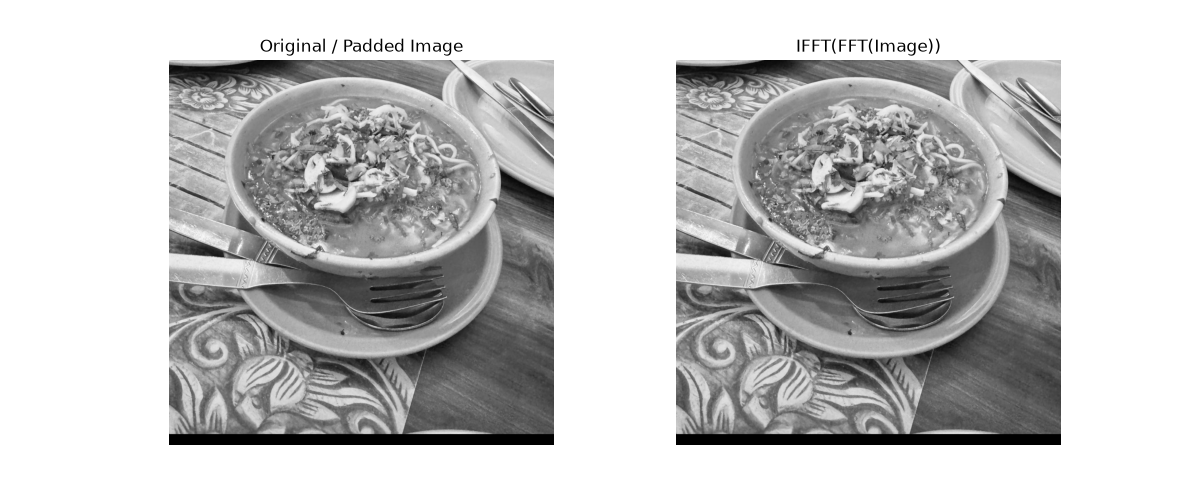
\includegraphics[width=0.8\linewidth]{part1_reconstruction.png}
    \caption{
    FFT verification. Left: original padded image.
    Right: reconstructed image after $IFFT(FFT(\text{Image}))$.
    }
    \label{fig:reconstruction}
\end{figure}


\subsection{Frequency-Domain Filtering}

We used a normalized $31\times31$ Gaussian kernel to blur the image. By the convolution theorem,

\[
f*h
\quad\longleftrightarrow\quad
F\cdot H,
\]

so the blurred image can be obtained as

\[
g=
\mathcal{F}^{-1}(F\cdot H).
\]

The filtering procedure was:

\begin{enumerate}
    \item Zero-pad the image to $1024\times1024$.
    
    \item Embed the Gaussian kernel in an array of the same size and shift its center to $(0,0)$.
    
    \item Compute the FFTs:
    \[
    F=\mathcal{F}(f),
    \qquad
    H=\mathcal{F}(h).
    \]
    
    \item Multiply them element-wise:
    \[
    G=F\cdot H.
    \]
    
    \item Compute $\mathcal{F}^{-1}(G)$ and crop the result to the original image size.
\end{enumerate}

For visualization, the Fourier spectra were displayed using the log-magnitude

\[
S(u,v)=\log\left(1+|F(u,v)|\right),
\]

with the zero-frequency component shifted to the center.

\begin{figure}[H]
    \centering
    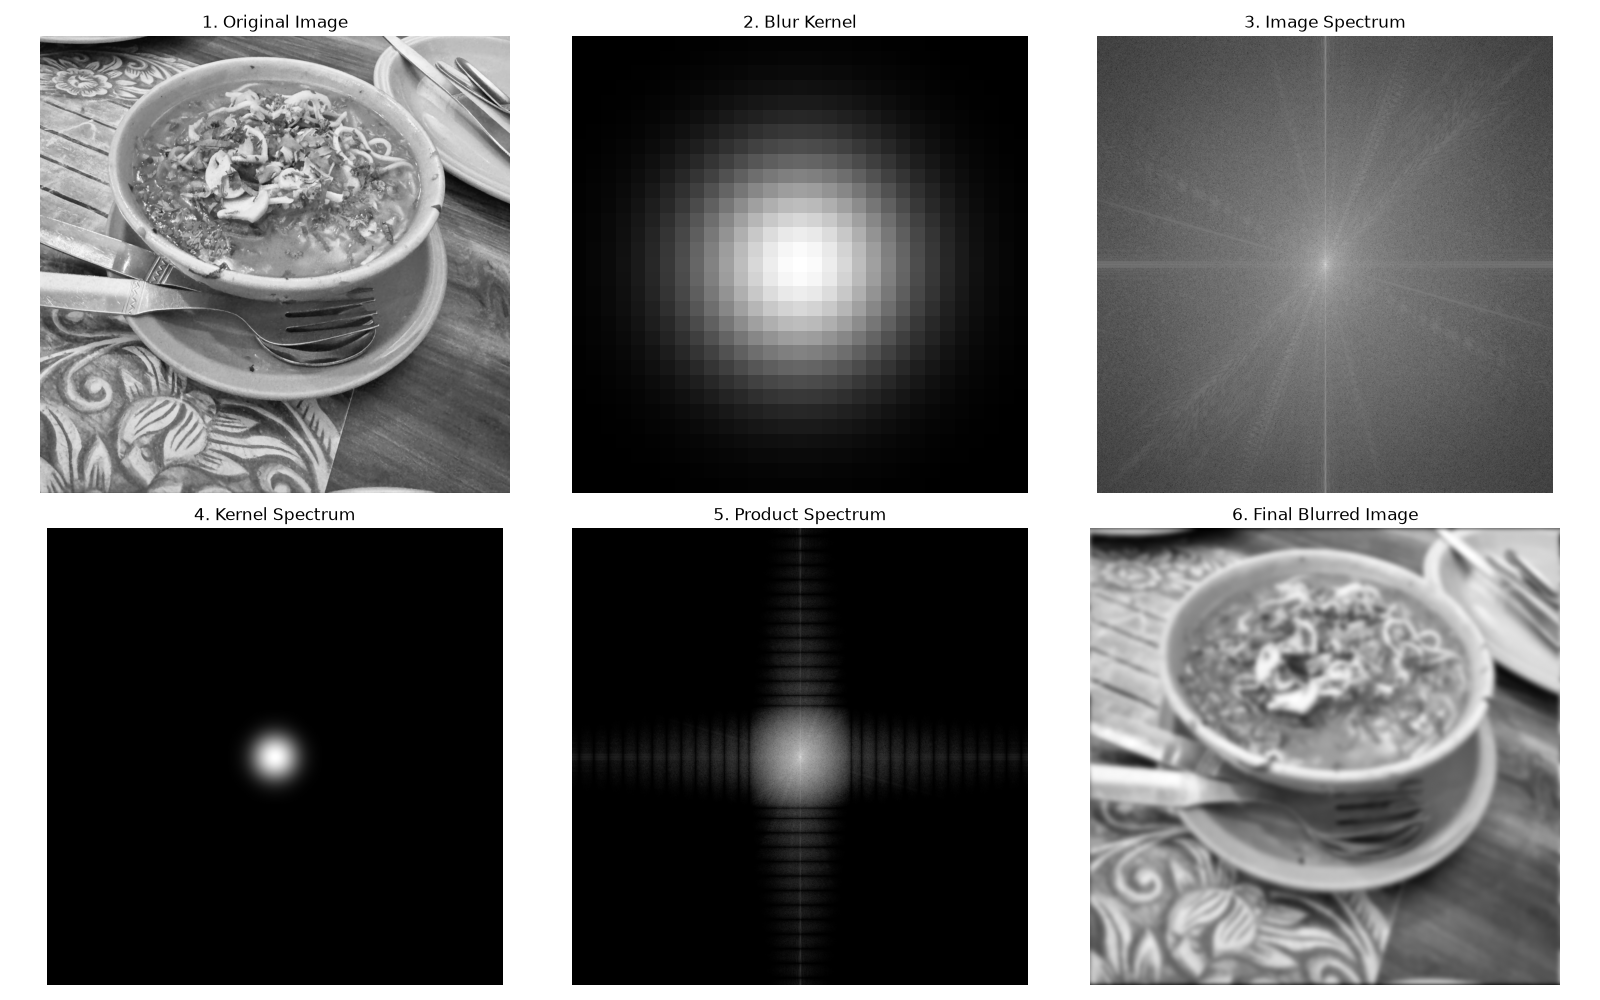
\includegraphics[width=1.0\linewidth]{part1_spectra_steps.png}
    \caption{
    Frequency-domain filtering steps: (1) original padded image,
    (2) Gaussian kernel, (3) image spectrum, (4) kernel spectrum,
    (5) product spectrum, and (6) final blurred image.
    }
    \label{fig:spectra_steps}
\end{figure}

The Gaussian spectrum is concentrated around low frequencies, showing its low-pass behaviour. Multiplication with this spectrum suppresses high-frequency components and produces the blurred image.


\subsection{Performance Comparison}

\subsubsection{Experimental Setup}

To compare spatial and frequency-domain filtering, we tested Gaussian kernels of sizes

\[
3,\;31,\;71,\;121,\;201,\;301,\;401,\;501.
\]

A smaller $248\times256$ image was used for timing to keep the computation manageable with our explicit Python FFT implementation.

\subsubsection{Computational Complexity}

For an $N\times N$ image and an $M\times M$ kernel, direct spatial convolution has complexity

\[
\mathcal{O}(N^2M^2).
\]

The frequency-domain approach requires 2D FFTs with complexity approximately

\[
\mathcal{O}(N^2\log N),
\]

plus element-wise multiplication. For a fixed image size, this cost is largely independent of the kernel size because the kernel is padded to the image dimensions.

\begin{figure}[H]
    \centering

    \begin{subfigure}[b]{0.48\textwidth}
        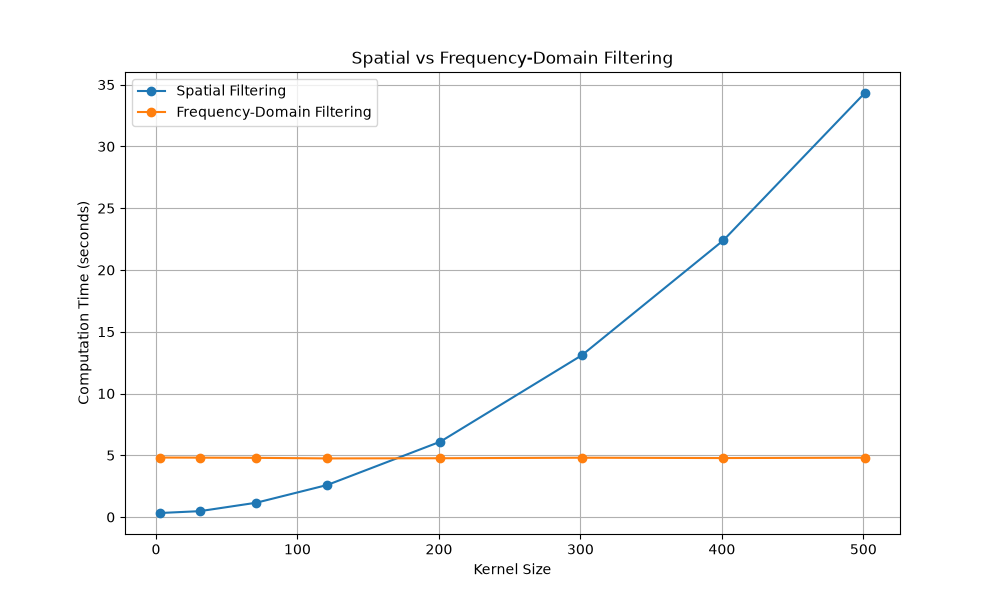
\includegraphics[width=\textwidth]{part1_time_comparison_linear.png}
        \caption{Linear Scale}
    \end{subfigure}
    \hfill
    \begin{subfigure}[b]{0.48\textwidth}
        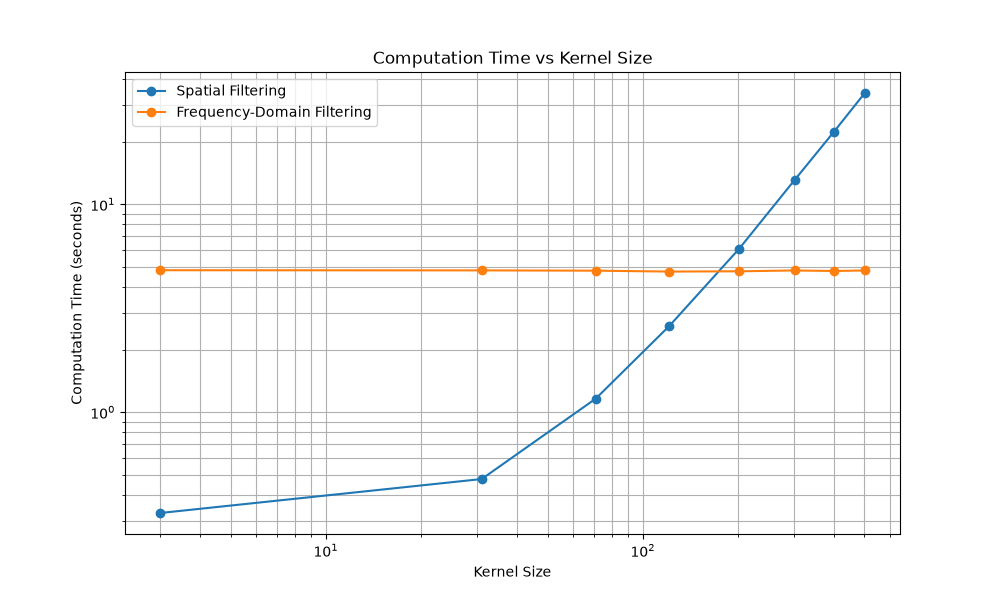
\includegraphics[width=\textwidth]{part1_time_comparison_loglog.png}
        \caption{Log-Log Scale}
    \end{subfigure}

    \caption{
    Computation time versus kernel size for spatial and frequency-domain
    filtering using a $248\times256$ image.
    }
    \label{fig:time_comparison}
\end{figure}

\subsubsection{Analysis of Performance Results}

The timing results in Figure~\ref{fig:time_comparison} show the different dependence of the two methods on kernel size.

\begin{itemize}
    \item \textbf{Spatial Filtering:}
    The computation time increases rapidly with kernel size because the number of operations per pixel scales as $M^2$. For the tested image, the time increased from approximately $0.08$ seconds for a $3\times3$ kernel to roughly $10$ seconds for a $501\times501$ kernel.

    \item \textbf{Frequency-Domain Filtering:}
    The computation time remains approximately constant at around $1.18$ seconds across the tested kernel sizes. This is because the FFT is performed on the fixed image-sized arrays, regardless of the kernel size.
\end{itemize}

For small kernels, spatial filtering is faster due to the overhead of the FFT. However, as the kernel becomes larger, its quadratic cost causes spatial filtering to become significantly slower. The results therefore demonstrate the advantage of frequency-domain filtering for sufficiently large kernels.

\subsection{Algorithm Pseudocode}
\begin{lstlisting}[
    language=Python,
    caption={Pseudo-code for FFT and Frequency-Domain Filtering},
    label={lst:part1}
]
INPUT: Grayscale image I, Kernel h
Pad I to power of two dimensions -> I_padded

/* 1A: 2D FFT */
F = Custom_FFT2D(I_padded)

/* 1B: Inverse 2D FFT and Verification */
I_reconstructed = Custom_IFFT2D(F)
Error = MAX(abs(I_padded - I_reconstructed))

/* 1C: Frequency-Domain Filtering */
Pad h to dimensions of I_padded
Shift h center to (0,0)
H = Custom_FFT2D(h_padded)

G = F * H
I_blurred = Custom_IFFT2D(G)
Crop I_blurred to original dimensions
\end{lstlisting}

\clearpage




\section{Part 2: Frequency Domain Analysis and Periodic Noise Removal}

This section explores frequency domain image processing techniques, focusing on the effects of sub-Nyquist sampling (aliasing), the design of anti-aliasing low-pass filters, and the removal of periodic interference patterns using notch filters. A custom implementation of the 2D Fast Fourier Transform (FFT) is utilized to compute the frequency spectra and apply the spatial filters in the frequency domain.

\subsection{Fourier Spectrum Analysis}

The initial objective is to analyze the frequency composition of an image containing a high-frequency repeating pattern. The input image is converted to grayscale, padded to the nearest power of two to satisfy the constraints of the radix-2 Cooley-Tukey algorithm, and transformed into the frequency domain.

\begin{figure}[H]
    \centering
    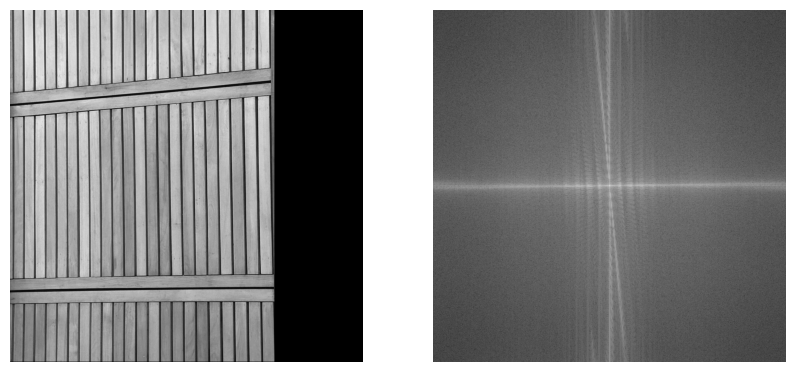
\includegraphics[width=0.8\textwidth]{part2_fig_a.png}
    \caption{Left: Original image padded to a power of two. Right: The Fourier magnitude spectrum displayed on a logarithmic scale. Distinct bright spikes (impulses) located away from the DC center component visually indicate the presence of strong periodic structural patterns.}
    \label{fig:spectrum_original}
\end{figure}

The Fourier spectrum clearly reveals the periodicity of the underlying pattern. The primary energy is concentrated in distinct impulses corresponding to the dominant spatial frequencies of the repetitive texture.

\subsection{Image Resampling and Aliasing}


When an image is downscaled through basic spatial subsampling without prior filtering, high-frequency components that exceed the new Nyquist limit are folded back into the lower frequencies. This phenomenon is known as aliasing.

To demonstrate this, the original image is spatially subsampled by a factor of $0.25$ using a nearest-neighbor approach. 



The subsampling process evidently violates the Nyquist-Shannon sampling theorem, resulting in severe structural distortion where the high-frequency repeating pattern masquerades as an artificial, low-frequency wave pattern.

\begin{figure}[H]
    \centering
    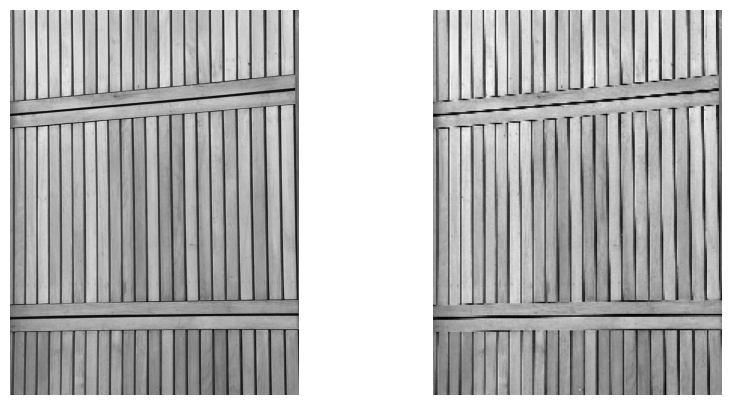
\includegraphics[width=0.8\textwidth]{part2_fig_b.png}
    \caption{Left: The original full-resolution image. Right: The resampled image demonstrating significant aliasing artifacts. The repeating pattern breaks down into visually distorted, lower-frequency moiré patterns.}
    \label{fig:aliasing}
\end{figure}

\subsection{Anti-Aliasing via Low-Pass Filtering}

\begin{figure}[H]
    \centering
    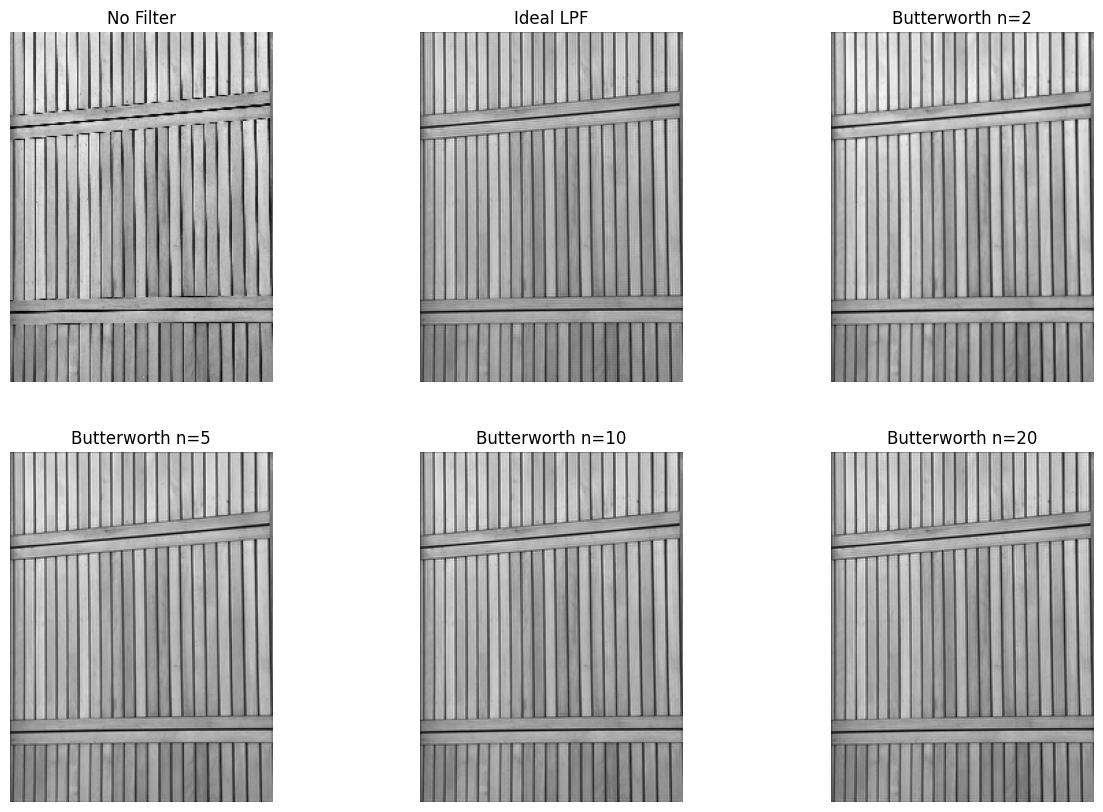
\includegraphics[width=0.95\textwidth]{part2_fig_c.png}
    \caption{Comparison of anti-aliasing filters prior to downsampling. The ideal LPF eliminates aliasing completely but introduces ringing (Gibbs phenomenon). As the Butterworth order $n$ increases, the result converges toward the ideal LPF.}
    \label{fig:lpf_comparison}
\end{figure}

Mathematically, subsampling an image by a factor of $M$ reduces the Nyquist frequency to $f_s / (2M)$. To prevent aliasing, signal frequencies exceeding this new Nyquist limit must be attenuated prior to subsampling. Consequently, the ideal low-pass filter (LPF) $H(u,v)$ in the frequency domain is defined as a 2D rectangular function:

\begin{equation}
H(u,v) = \begin{cases} 
1 & \text{if } |u| \le u_{max} \text{ and } |v| \le v_{max} \\
0 & \text{otherwise}
\end{cases}
\end{equation}

where $u_{max}$ and $v_{max}$ represent the strict Nyquist limits for the vertical and horizontal spatial frequencies, respectively.

To mitigate the ringing artifacts associated with the sharp cutoff of an ideal LPF, separable Butterworth low-pass filters are also evaluated. The transfer function of a separable Butterworth filter of order $n$ is defined as:

\begin{equation}
H_B(u,v) = \frac{1}{1 + (u/u_0)^{2n}} \times \frac{1}{1 + (v/v_0)^{2n}}
\end{equation}



\textbf{Analysis of Filter Quality and Artifacts:}
The ideal low-pass filter eliminates aliasing entirely; however, the sharp cutoff in the frequency domain introduces severe ringing artifacts in the spatial domain. The Butterworth filter provides a continuous transition between the passband and stopband. Lower-order Butterworth filters (e.g., $n=2, 5$) exhibit minimal ringing but provide insufficient attenuation of aliasing frequencies. Conversely, higher-order filters (e.g., $n=20$) effectively suppress aliasing but introduce pronounced spatial ringing artifacts, approaching the behavior of the ideal filter.

\subsection{Notch-Reject Filter Design}

\begin{figure}[H]
    \centering
    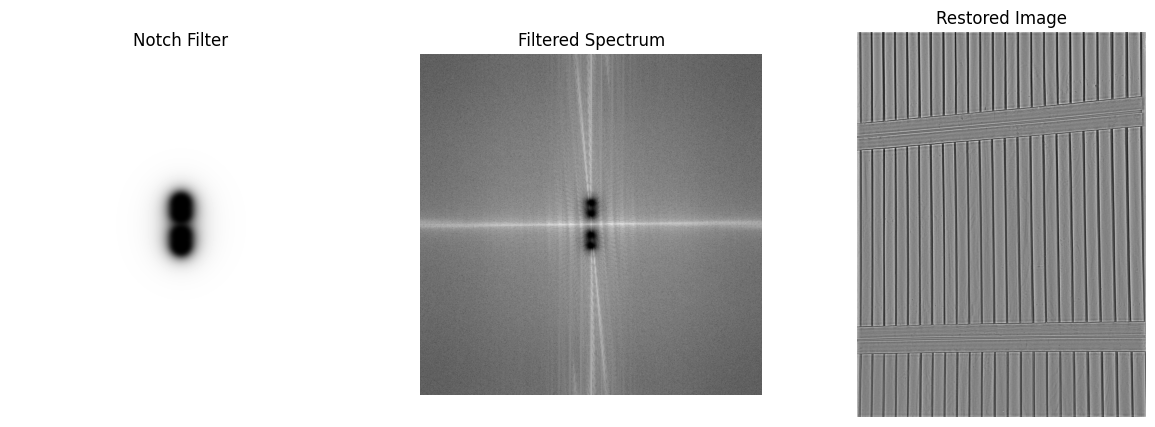
\includegraphics[width=0.95\textwidth]{part2_fig_d.png}
    \caption{Left: The synthesized notch transfer function $H(u,v)$. Middle: The filtered logarithmic spectrum. Right: The restored image with the periodic interference effectively suppressed.}
    \label{fig:notch_filter}
\end{figure}

To preserve original spatial dimensions while suppressing specific periodic noise patterns, a notch-reject filter is designed. The filter targets the distinct impulsive peaks identified in the frequency domain in Section 2.1.

The magnitude spectrum is computed, and the indices corresponding to the highest energy peaks (excluding the central DC component) are extracted. Conjugate symmetry is enforced to ensure the spatial output remains real-valued. A Butterworth notch-reject topology is employed to construct the transfer function:

\begin{equation}
H_{notch}(u,v) = \prod_{k=1}^{K} \left( \frac{1}{1 + (D_0 / D_k)^{2n}} \right) \left( \frac{1}{1 + (D_0 / D_{-k})^{2n}} \right)
\end{equation}

where $D_k$ and $D_{-k}$ represent the distance from the frequency coordinate $(u,v)$ to the identified symmetric notch centers $(u_k, v_k)$ and $(-u_k, -v_k)$, and $D_0$ is the notch radius.



\subsection{Optimum Notch Filtering}

\begin{figure}[H]
    \centering
    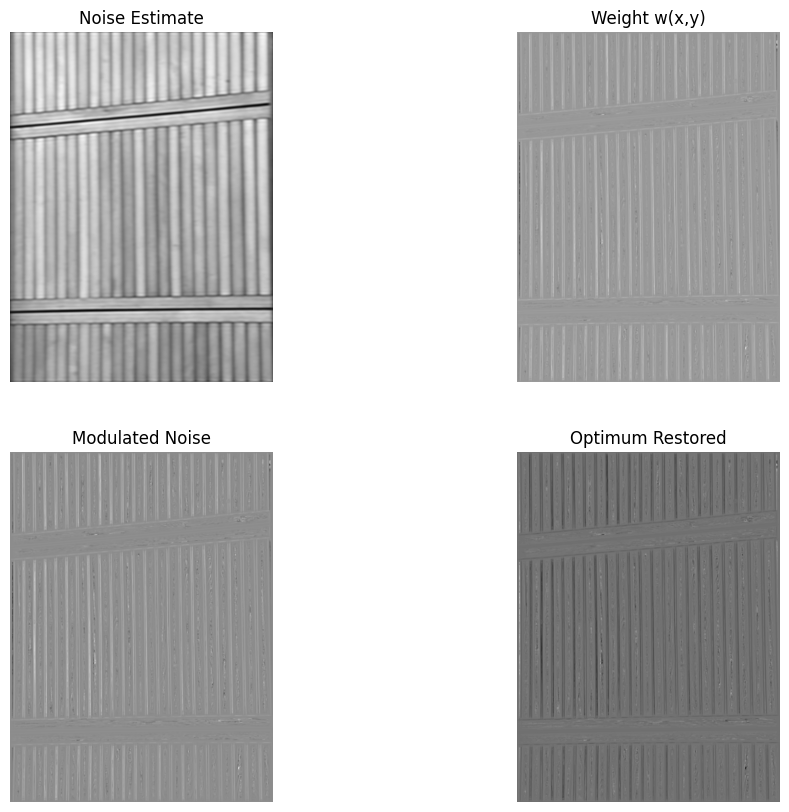
\includegraphics[width=0.85\textwidth]{part2_fig_e.png}
    \caption{Top Left: The isolated noise estimate $\eta(x,y)$. Top Right: The spatially adaptive weight function $w(x,y)$. Bottom Left: The modulated noise array. Bottom Right: The optimally restored output image.}
    \label{fig:optimum_notch}
\end{figure}

Standard notch filtering forcibly zeroes out specific frequency bands, which can inadvertently remove legitimate structural image information residing at those frequencies. Optimum notch filtering assumes that the periodic noise is additive and seeks to subtract a spatially modulated variant of the noise estimate from the original image, thereby minimizing local degradation.

The interference pattern is first isolated using a complementary Notch Pass Filter:
\begin{equation}
\eta(x,y) = \mathcal{F}^{-1}\{F(u,v) \cdot (1 - H_{notch}(u,v))\}
\end{equation}

A spatial neighborhood dimension (e.g., $5 \times 5$) is established to compute local variance and covariance estimators using a uniform box filter. A spatially adaptive weight function $w(x,y)$ is derived:

\begin{equation}
w(x,y) = \frac{\text{cov}(f(x,y), \eta(x,y))}{\text{var}(\eta(x,y)) + \epsilon}
\end{equation}

The modulated noise estimate is subsequently deducted from the original degraded image:

\begin{equation}
f_{restored}(x,y) = f_{degraded}(x,y) - w(x,y) \eta(x,y)
\end{equation}



\textbf{Analysis of Local Neighborhood Size:}
The selection of the local neighborhood dimension fundamentally dictates the accuracy of the local variance and covariance estimators. A neighborhood size that is excessively small causes the weight function $w(x,y)$ to become highly sensitive to microscopic intensity fluctuations, propagating spurious modulation artifacts into the restored image. Conversely, an excessively large neighborhood homogenizes the estimators, causing the weight function to lose spatial adaptability. In such cases, the algorithm fails to distinguish between the periodic interference pattern and legitimate high-contrast image structures. An optimal neighborhood size mitigates these extremes, facilitating a spatially adaptive subtraction that suppresses periodic noise without eroding intrinsic structural details.

\subsection{Algorithm Pseudocode}
\begin{lstlisting}[
    language=Python,
    caption={Pseudo-code for Frequency Domain Filtering and Optimal Notch Reconstruction},
    label={lst:part2}
]
INPUT: Degraded grayscale image I
Pad I to nearest power of two dimensions -> I_padded

/* 2A: Forward Transform */
F = Custom_FFT2D(I_padded)
F_shifted = FFTShift(F)

/* 2B: Basic Subsampling (Aliasing demonstration) */
I_resampled = I[::4, ::4]

/* 2C: Anti-Aliasing Low-Pass Filters */
Generate Ideal_Rect_Filter matching downsample Nyquist bounds
F_ideal = F_shifted * Ideal_Rect_Filter
I_ideal_anti_aliased = Custom_IFFT2D(F_ideal)

FOR order n IN [2, 5, 10, 20]:
    Generate Butterworth_Filter of order n
    F_bw = F_shifted * Butterworth_Filter
    I_bw_anti_aliased = Custom_IFFT2D(F_bw)

/* 2D: Standard Notch-Reject Filtering */
Identify Top K frequency impulse coordinates (excluding DC)
Construct H_notch Butterworth filter targeting identified coordinates

F_notch = F_shifted * H_notch
I_notch_restored = Custom_IFFT2D(F_notch)

/* 2E: Optimal Notch Filtering */
H_notch_pass = 1.0 - H_notch
F_noise = F_shifted * H_notch_pass
Noise_Estimate = Custom_IFFT2D(F_noise)

Define BoxFilter(Window=5)
Mean_Noise = BoxFilter(Noise_Estimate)
Mean_Image = BoxFilter(I_padded)

Var_Noise = BoxFilter(Noise_Estimate^2) - Mean_Noise^2
Cov_Img_Noise = BoxFilter(I_padded * Noise_Estimate) - (Mean_Image * Mean_Noise)

Weight_Map(w) = Cov_Img_Noise / (Var_Noise + epsilon)
I_optimal_restored = I_padded - (w * Noise_Estimate)

Crop padding and save outputs
\end{lstlisting}


\clearpage




\section{Part 3: Image Denoising and Wiener Filtering}

This section evaluates techniques for noise variance estimation, spatial filtering (arithmetic mean and median), and frequency-domain Wiener filtering on a reference image degraded by additive white Gaussian noise. 

\subsection{Image Acquisition and Synthetic Noise Injection}

A reference image (\texttt{kodim04.png}) from the Kodak image suite is acquired and converted to grayscale. Synthetic Gaussian noise is injected such that the Peak Signal-to-Noise Ratio (PSNR) is exactly $20$ dB. The noisy image intensity values are deliberately unclipped, allowing them to exceed the standard $[0, 255]$ dynamic boundary to maintain linear noise statistics.

\begin{figure}[H]
    \centering
    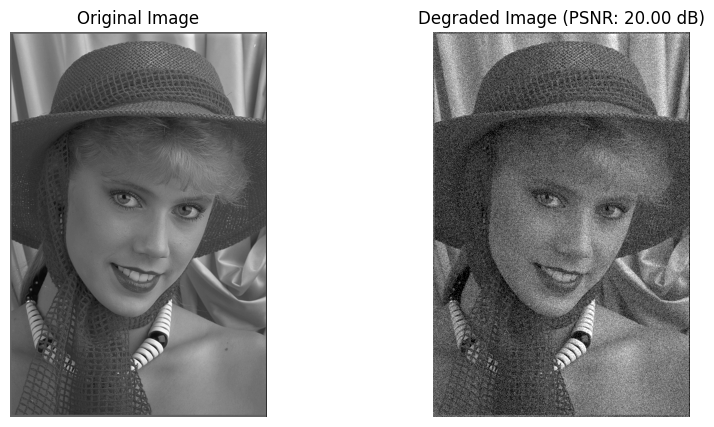
\includegraphics[width=0.85\textwidth]{part3_fig_a.png}
    \caption{Left: The original uncorrupted Kodak reference image. Right: The image degraded with synthetic additive white Gaussian noise (PSNR exactly $20$ dB).}
    \label{fig:noise_injection}
\end{figure}

The true noise variance required to achieve a $20$ dB PSNR is calculated analytically as $\sigma^2 = 255^2 / 100 \approx 650.25$. 

\subsection{Blind Noise Variance Estimation}

In the absence of a priori knowledge regarding the noise statistics, the noise variance is estimated directly from the degraded image. A computationally efficient and robust estimation method involves partitioning the image into small non-overlapping spatial blocks (e.g., $16 \times 16$) and calculating the sample variance within each block. 

Under the assumption that the natural image contains at least one completely smooth, textureless region, the intrinsic structural variance of that optimal region approaches zero. Consequently, the minimum variance observed across all spatial blocks serves as an effective empirical estimate of the global noise variance. This procedure yields an estimated variance that closely matches the theoretical true variance ($\sigma^2 \approx 650.25$).

\subsection{Spatial Filtering: Arithmetic Mean and Median Filters}

The degraded image is subjected to spatial denoising using $m \times m$ arithmetic mean and median filters. To avoid external high-level image processing libraries, vectorized spatial window extraction is utilized via array stride manipulation. The PSNR is computed for filter sizes $m \in \{1, 3, 5, 7, 9\}$.

\begin{figure}[H]
    \centering
    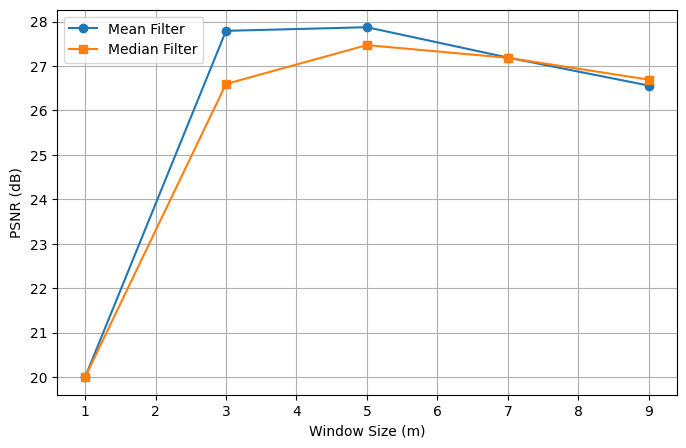
\includegraphics[width=0.65\textwidth]{part3_fig_b.png}
    \caption{Denoising performance (PSNR) plotted as a function of the spatial filter window size $m$ for both arithmetic mean and median filters.}
    \label{fig:spatial_psnr}
\end{figure}

\textbf{Analysis of PSNR Dynamics with Respect to Filter Size:}
Spatial filters operate by aggregating local neighborhood information. Initially, increasing the spatial window size $m$ incorporates more neighborhood samples, effectively averaging out the zero-mean independent Gaussian noise. This substantially reduces the residual noise variance and yields a corresponding increase in the PSNR. 

However, as $m$ continues to expand, the filters process increasingly heterogeneous spatial regions, resulting in the progressive blurring of high-frequency structural details (such as edges and textures). Eventually, the structural degradation penalty outweighs the noise reduction benefits, causing the Mean Squared Error (MSE) to rise and the overall PSNR to decline.

\begin{figure}[H]
    \centering
    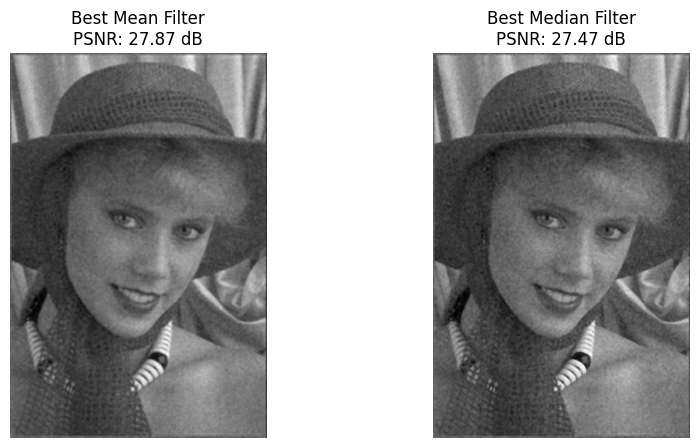
\includegraphics[width=0.85\textwidth]{part3_fig_c.png}
    \caption{The optimally restored images for both spatial filtering techniques. Left: Best Mean Filter result. Right: Best Median Filter result.}
    \label{fig:best_spatial}
\end{figure}

\subsection{Frequency-Domain Wiener Filtering}

The Wiener filter minimizes the mean square error between the estimated image and the true image. In the frequency domain, the Wiener filter transfer function without blur is formulated as:

\begin{equation}
W(u,v) = \frac{S_f(u,v)}{S_f(u,v) + S_\eta(u,v)} = \frac{1}{1 + \frac{S_\eta(u,v)}{S_f(u,v)}}
\end{equation}

where $S_f$ and $S_\eta$ represent the power spectral densities of the image and the noise, respectively.

\subsubsection{Constant Power Spectral Density Ratio Assumption}
When the ratio $S_\eta / S_f$ is strictly assumed to be a global constant $K$, the transfer function simplifies to $W(u,v) = \frac{1}{1 + K}$. Under this assumption, the filter operates purely as a uniform scalar multiplier across all frequencies, scaling down both signal and noise proportionally. A parameter sweep identifies the empirical optimum constant $K$ that maximizes the PSNR.

\subsubsection{Frequency-Dependent Adaptive Estimate}
A robust frequency-dependent estimate leverages the expected noise power spectrum. For Gaussian white noise, $\mathbb{E}(|N[u,v]|^2) \approx M N \sigma^2$, where $M, N$ correspond to the spatial dimensions of the padded image. The uncorrupted image power spectrum is approximated via spectral subtraction: 

\begin{equation}
\mathbb{E}(|F[u,v]|^2) \approx \max(|G[u,v]|^2 - \mathbb{E}(|N[u,v]|^2), 0)
\end{equation}

Substituting this into the formulation yields a frequency-adaptive filter that attenuates individual frequency bins selectively based on their localized signal-to-noise ratio.

\begin{figure}[H]
    \centering
    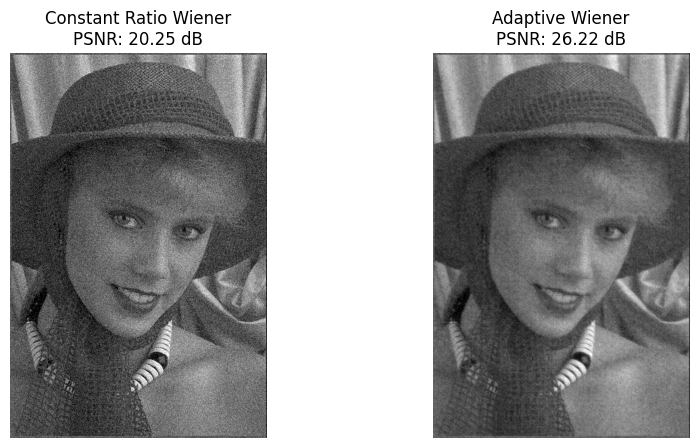
\includegraphics[width=0.85\textwidth]{part3_fig_d.png}
    \caption{Left: The result of the Constant Ratio Wiener Filter, optimized via grid search over $K$. Right: The result of the Frequency-Dependent Adaptive Wiener Filter. The adaptive filter preserves high-frequency structural details significantly better than the constant scalar approach.}
    \label{fig:wiener_comparison}
\end{figure}

\subsection{Algorithm Pseudocode}
\begin{lstlisting}[
    language=Python,
    caption={Pseudo-code for Noise Estimation and Wiener Filtering},
    label={lst:part3}
]
INPUT: Clean reference image I
Calculate sigma for target 20dB PSNR
Noise = Generate_Gaussian_Noise(sigma)
I_degraded = I + Noise

/* 3A: Blind Noise Estimation */
Min_Variance = Infinity
FOR each non-overlapping 16x16 block IN I_degraded:
    IF Var(block) < Min_Variance:
        Min_Variance = Var(block)
Estimated_Variance = Min_Variance

/* 3B: Spatial Filtering */
FOR m IN [1, 3, 5, 7, 9]:
    I_mean = Custom_MeanFilter(I_degraded, m)
    I_median = Custom_MedianFilter(I_degraded, m)
    Record PSNR for both filters
Plot PSNR vs m and select best m

/* 3C: Wiener Filtering (Constant Ratio) */
Pad I_degraded to power of two dimensions
G = Custom_FFT2D(I_degraded_padded)

Best_PSNR = 0
FOR K in logarithmic_space:
    W_constant = 1 / (1 + K)
    F_hat = G * W_constant
    I_restored = Custom_IFFT2D(F_hat)
    IF PSNR(I_restored) > Best_PSNR: Best_K = K

/* 3D: Wiener Filtering (Adaptive Frequency-Dependent) */
M, N = Dimensions(G)
Expected_Noise_Power = M * N * Estimated_Variance
Power_Spectrum_G = abs(G)^2

Estimated_F_Power = MAX(Power_Spectrum_G - Expected_Noise_Power, 0)
W_adaptive = Estimated_F_Power / (Estimated_F_Power + Expected_Noise_Power)

F_hat_adaptive = G * W_adaptive
I_adaptive_restored = Custom_IFFT2D(F_hat_adaptive)

Display comparative results
\end{lstlisting}


\clearpage




\section{Part 4: Frequency-Domain Filtering and Image Restoration}

% =========================================================
\subsection{Motion Blur Estimation and Transfer Function}
% =========================================================

\subsubsection{Estimating the Blur Vector}

The image was captured while rotating the camera, producing predominantly horizontal motion blur. We model the motion as

\[
x_0(t)=at,\qquad y_0(t)=bt,\qquad t\in[0,1].
\]

By examining the length and direction of the visible streaks, we estimated the blur to be approximately 30 pixels horizontally, with negligible vertical motion. Thus,

\[
\boxed{(a,b)=(30,0)\text{ pixels}.}
\]

\subsubsection{Transfer Function}

The blurred image is

\[
g(x,y)=\int_0^1 f(x-at,y-bt)\,dt.
\]

Taking the Fourier transform gives

\[
G(u,v)=H(u,v)F(u,v),
\]

where

\[
H(u,v)
=
\int_0^1 e^{-i2\pi(ua+vb)t}\,dt.
\]

Therefore,

\[
\boxed{
H(u,v)
=
e^{-i\pi(ua+vb)}
\operatorname{sinc}(ua+vb)
}
\]

where

\[
\operatorname{sinc}(x)=\frac{\sin(\pi x)}{\pi x}.
\]

For $(a,b)=(30,0)$,

\[
\boxed{
H(u,v)=e^{-i30\pi u}\operatorname{sinc}(30u)
}
\]

and hence

\[
\boxed{|H(u,v)|=|\operatorname{sinc}(30u)|.}
\]

Since the blur is horizontal, the zeros of $H$ form approximately vertical bands in the frequency domain.

\begin{figure}[H]
    \centering
    \begin{subfigure}[b]{0.45\textwidth}
        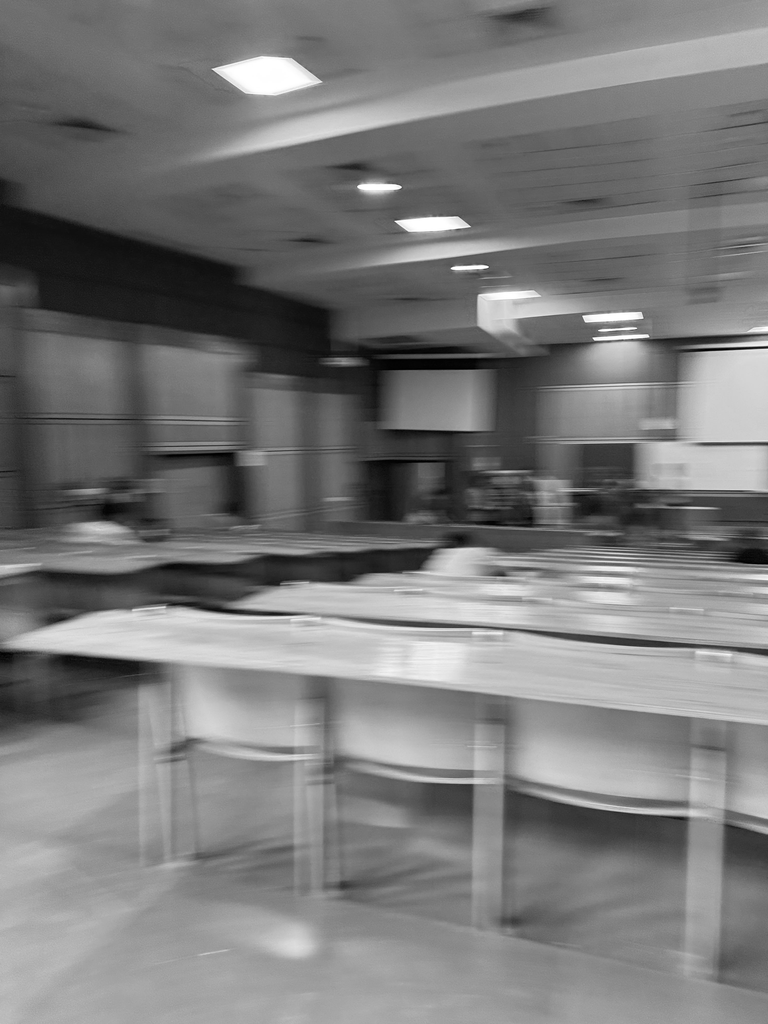
\includegraphics[width=\textwidth]{part4_01_input.png}
        \caption{Input blurred image}
    \end{subfigure}
    \hfill
    \begin{subfigure}[b]{0.45\textwidth}
        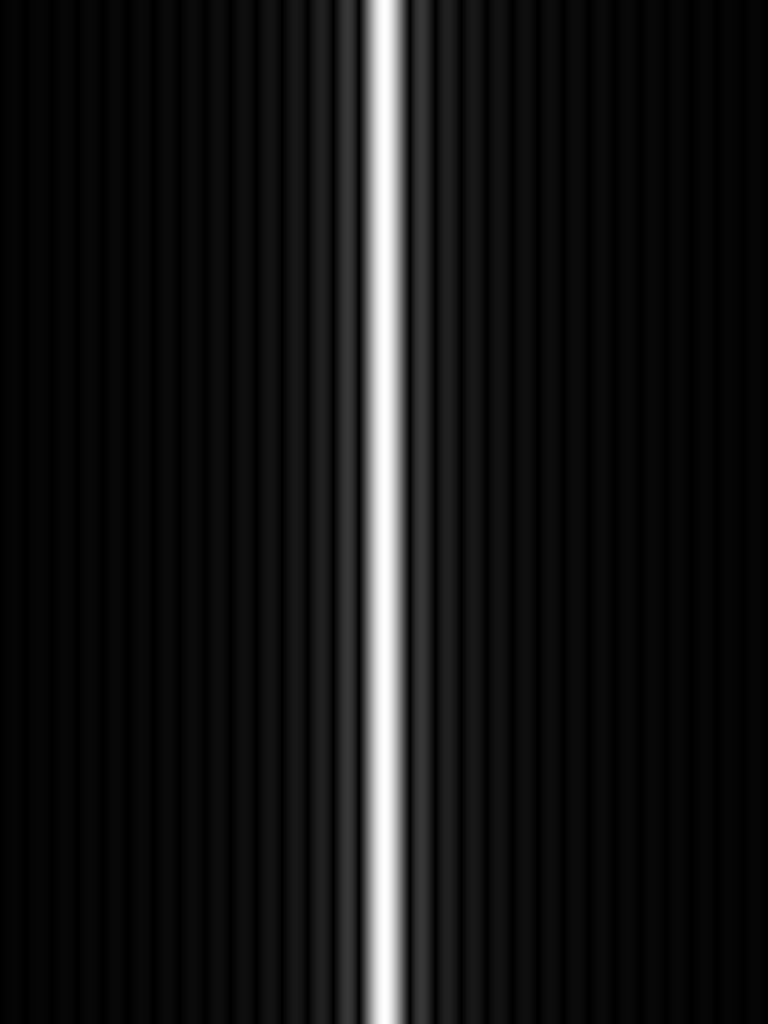
\includegraphics[width=\textwidth]{part4_02_H_magnitude.png}
        \caption{$|H(u,v)|$}
    \end{subfigure}
    \caption{Input image and magnitude of the motion-blur transfer function.}
\end{figure}

The Fourier spectrum shows the expected directional structure caused by the horizontal motion blur.

% =========================================================
\subsection{Inverse Filtering}
% =========================================================

Inverse filtering estimates the original spectrum as

\begin{figure}[H]
    \centering
    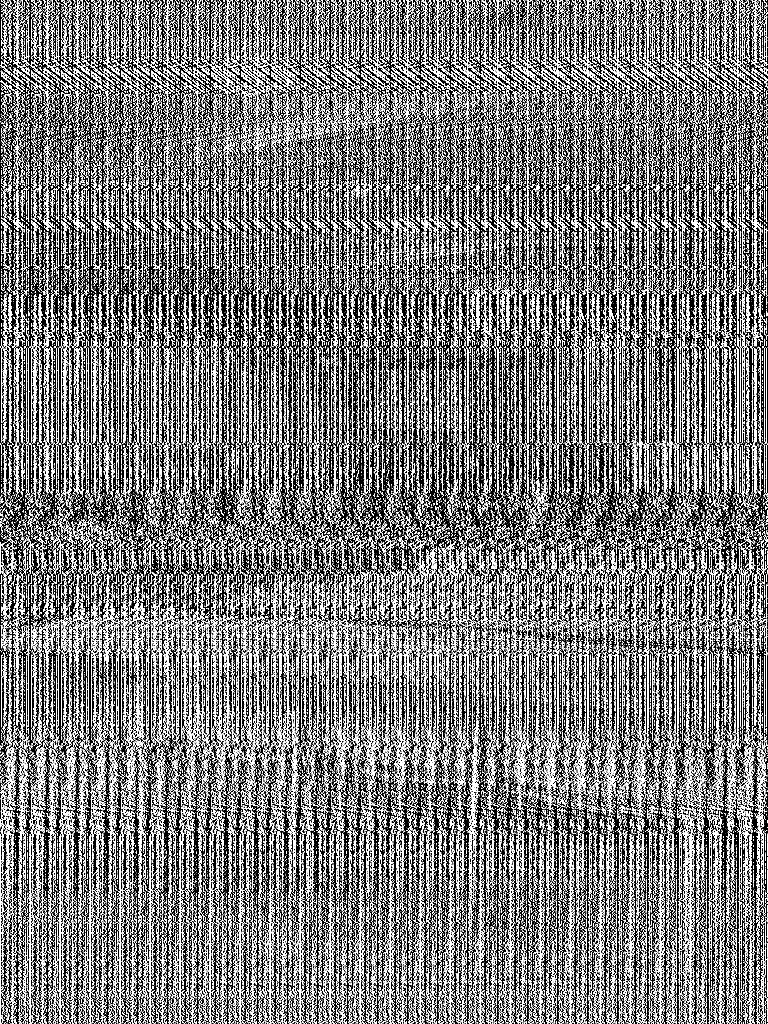
\includegraphics[width=0.35\linewidth]{part4_03_inverse_filter.png}
    \caption{Result of inverse filtering.}
\end{figure}
\[
\boxed{
\hat F(u,v)=\frac{G(u,v)}{H(u,v)}.
}
\]

Since $H$ has zeros, direct division is unstable. In the implementation, values satisfying

\[
|H(u,v)|<10^{-3}
\]

were replaced by $10^{-3}$.



The result contains severe streaking artifacts. This occurs because frequencies for which $|H|$ is small are strongly amplified by $1/H$, including noise and modelling errors. Since the problematic frequencies occur along specific bands rather than uniformly in the frequency plane, the resulting artifacts are directional rather than isotropic.

% =========================================================
\subsection{Wiener Deconvolution}
% =========================================================

To reduce the instability of inverse filtering, we used the Wiener filter

\[
\boxed{
\hat F(u,v)
=
\frac{H^*(u,v)}
{|H(u,v)|^2+K}G(u,v).
}
\]

We tested a range of $K$ values. Small values produced strong streaking, while large values excessively smoothed the image. Based on visual comparison, we selected

\[
\boxed{K_{\mathrm{best}}=0.005}.
\]

The required comparison is therefore

\[
0.1K=0.0005,\qquad
K=0.005,\qquad
10K=0.05.
\]

\begin{figure}[H]
    \centering
    \begin{subfigure}[b]{0.32\textwidth}
        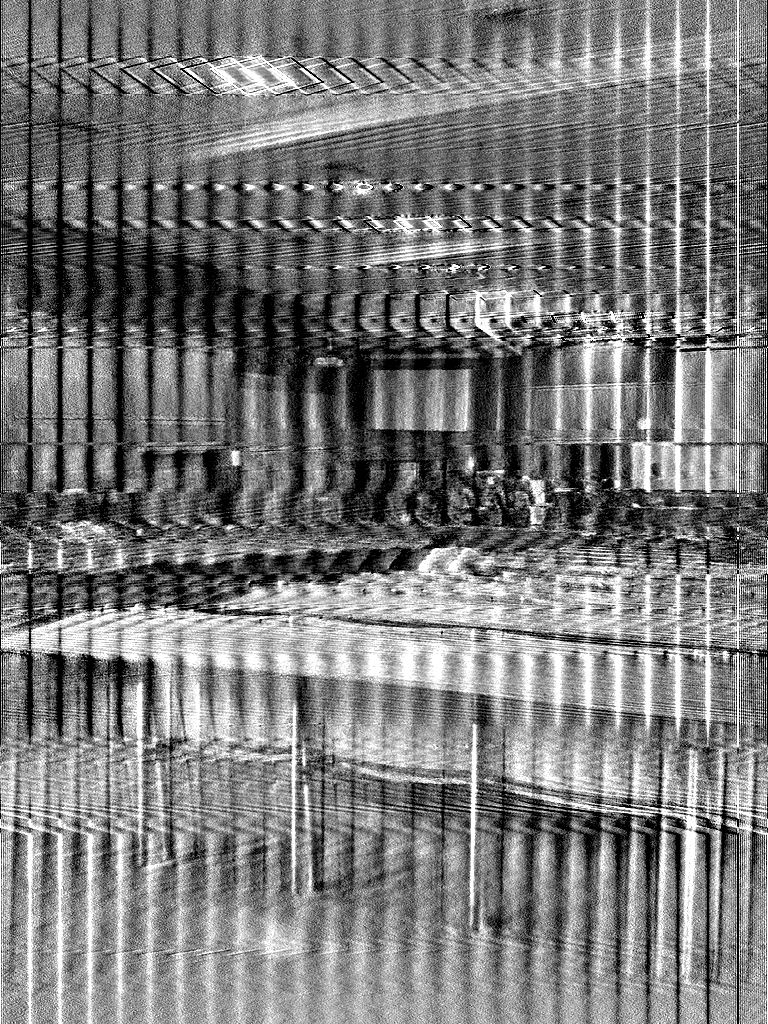
\includegraphics[width=\textwidth]{part4_04_wiener_0.1K.png}
        \caption{$K=0.0005$}
    \end{subfigure}
    \hfill
    \begin{subfigure}[b]{0.32\textwidth}
        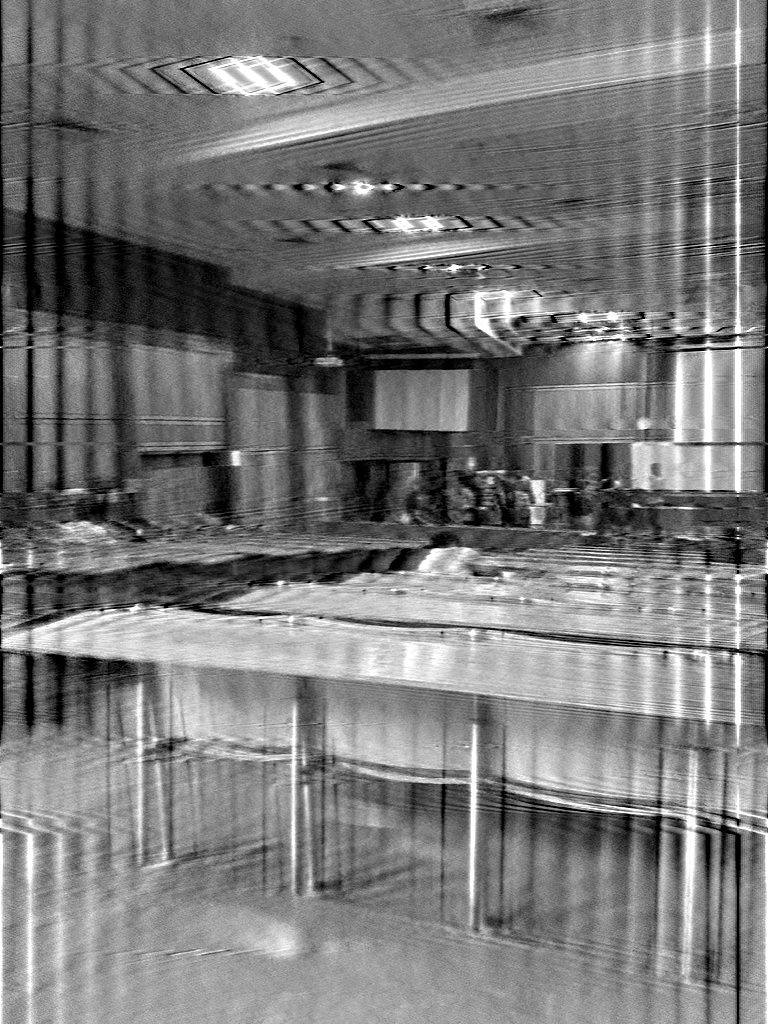
\includegraphics[width=\textwidth]{part4_05_wiener_best.png}
        \caption{$K=0.005$}
    \end{subfigure}
    \hfill
    \begin{subfigure}[b]{0.32\textwidth}
        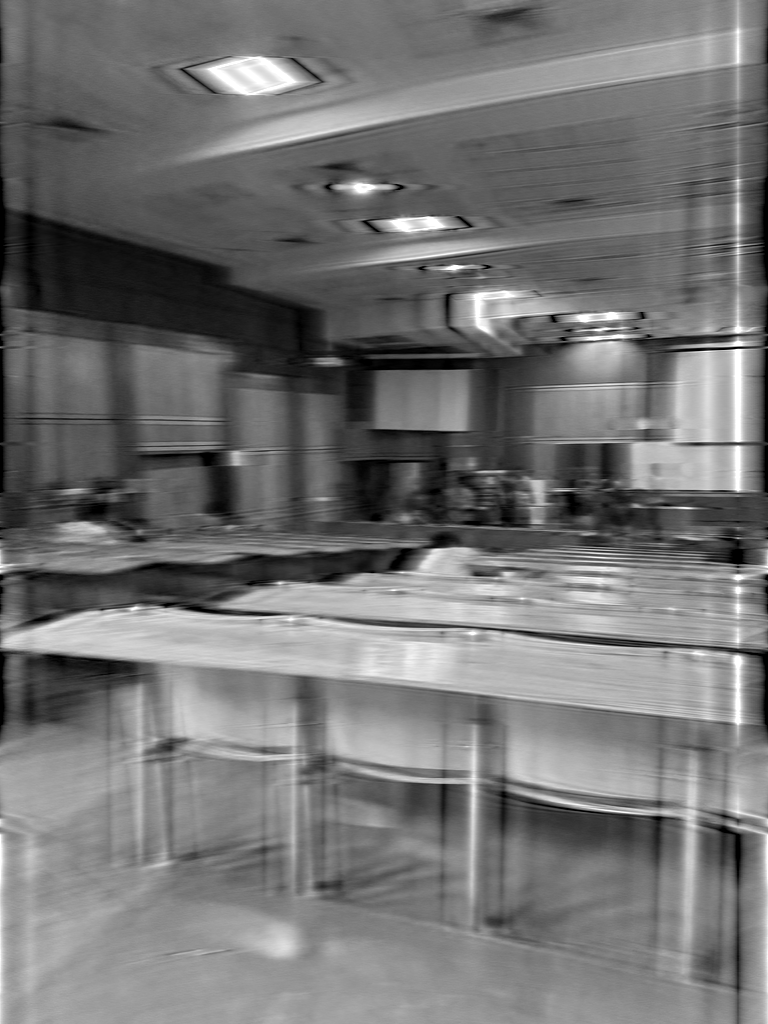
\includegraphics[width=\textwidth]{part4_06_wiener_10K.png}
        \caption{$K=0.05$}
    \end{subfigure}
    \caption{Wiener deconvolution for $0.1K$, $K$, and $10K$.}
\end{figure}

For $K=0.0005$, the restoration is extremely aggressive, but streaking noise completely dominates the image. At $K=0.005$, the image retains strong sharpness, but there are still distinct line artifacts present. These lines are ringing artifacts caused by the near-zero values of the transfer function $H(u,v)$ in the frequency domain. There is an inherent trade-off here: if we try to fully remove these lines by increasing the regularization further (e.g., to $K=0.05$), the artifacts successfully vanish, but the high-frequency details are also heavily suppressed, causing the overall image to become unacceptably blurry. Thus, $K=0.005$ gives the best qualitative compromise by maximizing the deblurring sharpness at the cost of retaining some of these artifact lines.

% =========================================================
\subsection{Regularized Deconvolution}
% =========================================================

\begin{figure}[H]
    \centering
    \begin{subfigure}[b]{0.32\textwidth}
        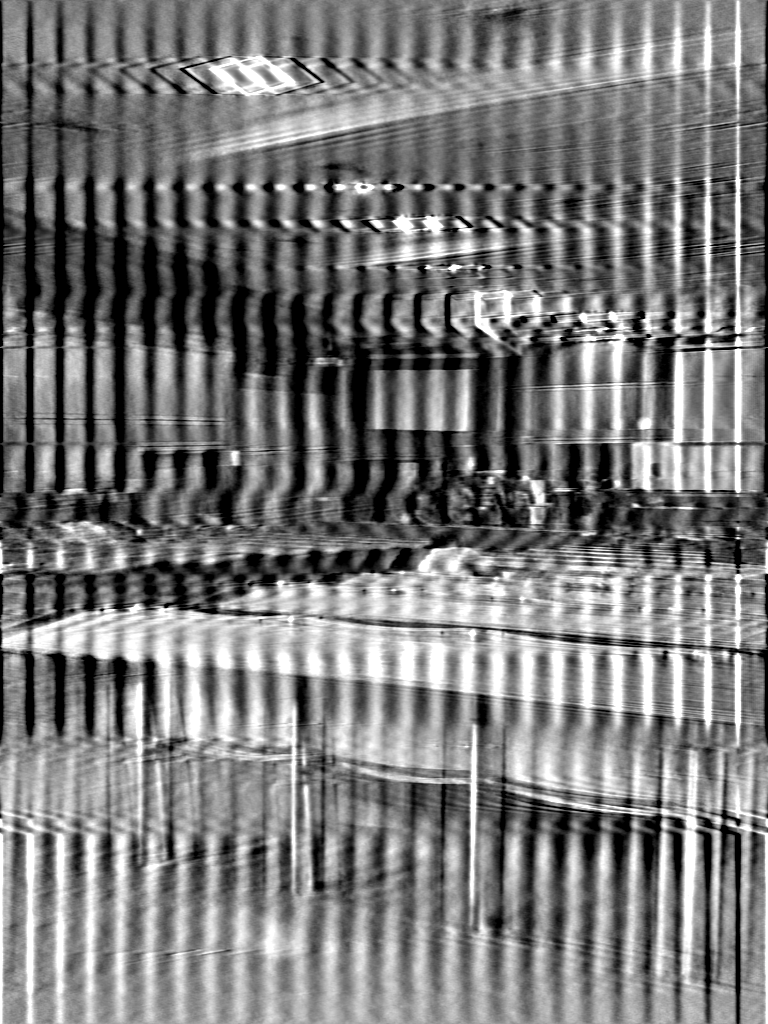
\includegraphics[width=\textwidth]{part4_07_reg_0.1lam.png}
        \caption{$0.1\lambda=0.005$}
    \end{subfigure}
    \hfill
    \begin{subfigure}[b]{0.32\textwidth}
        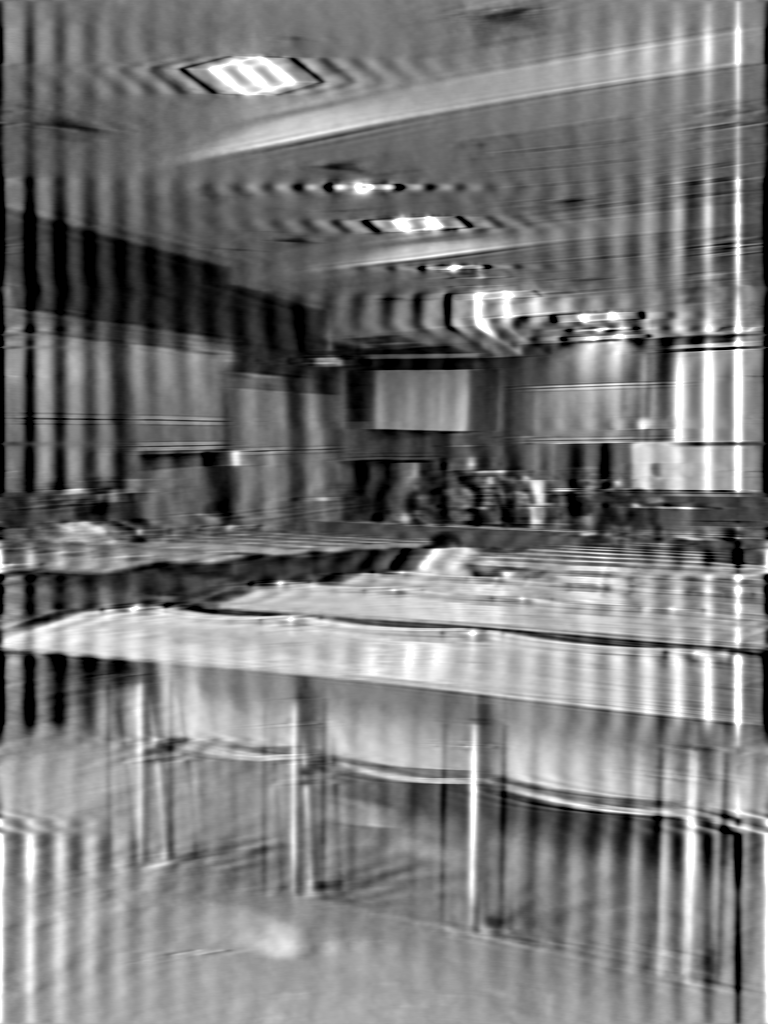
\includegraphics[width=\textwidth]{part4_08_reg_best.png}
        \caption{$\lambda=0.05$}
    \end{subfigure}
    \hfill
    \begin{subfigure}[b]{0.32\textwidth}
        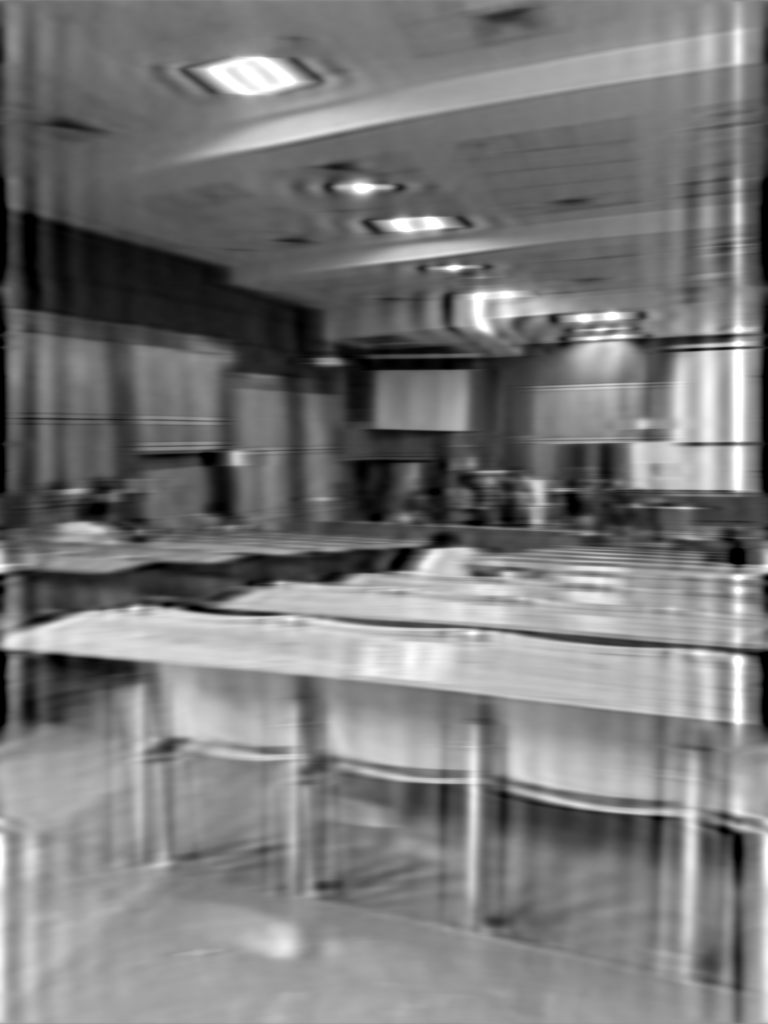
\includegraphics[width=\textwidth]{part4_09_reg_10lam.png}
        \caption{$10\lambda=0.5$}
    \end{subfigure}
    \caption{Regularized deconvolution for three values of $\lambda$.}
\end{figure}

We use the squared gradient norm specified in the assignment:

\[
R(\hat f)
=
\sum_{x,y}
\left[
(\hat f(x+1,y)-\hat f(x,y))^2+
(\hat f(x,y+1)-\hat f(x,y))^2
\right].
\]

The objective is

\[
E(\hat f)=\|h*\hat f-g\|^2+\lambda R(\hat f).
\]

For the finite differences,

\[
|D_x(u,v)|^2=4\sin^2(\pi u),
\qquad
|D_y(u,v)|^2=4\sin^2(\pi v).
\]

Thus,

\[
P(u,v)
=
4\sin^2(\pi u)+4\sin^2(\pi v).
\]

In the Fourier domain,

\[
E(\hat F)
=
\sum_{u,v}
\left[
|H\hat F-G|^2+
\lambda P|\hat F|^2
\right].
\]

Setting the derivative with respect to $\hat F^*$ to zero gives

\[
\boxed{
\hat F(u,v)
=
\frac{H^*(u,v)G(u,v)}
{|H(u,v)|^2+\lambda P(u,v)}
}
\]

or equivalently,

\[
\boxed{
\hat F(u,v)
=
\frac{H^*(u,v)G(u,v)}
{|H(u,v)|^2+
\lambda\left[
4\sin^2(\pi u)+4\sin^2(\pi v)
\right]}.
}
\]

We tested a wide range of $\lambda$ values and found

\[
\boxed{\lambda_{\mathrm{best}}=0.05}
\]

to give the best qualitative result.



With $\lambda=0.005$, more streaking remains due to weak regularization. At $\lambda=0.05$, the artifacts are substantially reduced while image structure is retained. For $\lambda=0.5$, stronger smoothing removes additional high-frequency detail. Hence, $\lambda=0.05$ was selected.

\subsection{Algorithm Pseudocode}
\begin{lstlisting}[
    language=Python,
    caption={Pseudo-code for Motion Blur Estimation and Restoration},
    label={lst:part4}
]
INPUT: Blurred image g
Pad g to power of two dimensions -> g_padded
G = Custom_FFT2D(g_padded)

/* 4A: Transfer Function */
Estimate blur parameters (a, b) = (30, 0)
H(u,v) = exp(-i*pi*(u*a + v*b)) * sinc(u*a + v*b)

/* 4B: Inverse Filtering */
H_inv = H
H_inv[abs(H_inv) < 1e-3] = 1e-3
F_hat_inverse = G / H_inv
I_inverse = Custom_IFFT2D(F_hat_inverse)

/* 4C: Wiener Deconvolution */
K_best = 0.005
W_wiener = conj(H) / (abs(H)^2 + K_best)
F_hat_wiener = G * W_wiener
I_wiener = Custom_IFFT2D(F_hat_wiener)

/* 4D: Regularized Deconvolution */
lambda_best = 0.05
P = 4*sin(pi*u)^2 + 4*sin(pi*v)^2
W_reg = conj(H) / (abs(H)^2 + lambda_best * P)
F_hat_reg = G * W_reg
I_reg = Custom_IFFT2D(F_hat_reg)

Crop restored images to original dimensions
\end{lstlisting}

\end{document}
